\subsection{Objective-conditioned joint code and graph search}

The next pilot returns to the central experimental object: change the loss,
then observe changes in the search path and executable system. It does not
first increase populations, seeds or the horizon. Scoped graph authoring
removes incidental global-name and phase bookkeeping: the designer explicitly
chooses Python implementations, node ordering, typed intermediate protocols,
input sources and native exports. A mechanical compiler namespaces local IDs
and assigns ordered phases inside the existing cut. It does not supply missing
semantic wires, replace invalid source or choose an institutional algorithm.

Two explicitly illustrative engineering objectives use real native outcomes:
\begin{align}
 L_{\mathrm{throughput}} &= -A,\\
 L_{\mathrm{net\ review}} &= 3.25A-Q+0.05R,
\end{align}
where $A$ counts actual acceptance decisions, $Q$ sums the raw reviewer-score
mean of each accepted decision, and $R$ counts actual reviews. The generated
institution's self-written final score cannot manufacture $Q$. Publication
and review charges are declared preferences, not calibrated scientific value.
Reject-all is allowed when this proxy rewards it; there is no hidden quality,
participation or fairness veto. Neither objective measures verified knowledge.
The charge 3.25 was chosen with earlier development scores of 3 in mind, before
this pilot, to expose a competing preference. A resulting contrast is therefore
illustrative, not an independent discovery of a normative trade-off.

Each arm starts from the same developer-authored rank/rate selection slot and
has two adaptive slots, with at most three technical drafts per slot. First
source is withheld; subsequent prompts include actual loss/measurements and
the exact previously generated code, protocols and wiring, including a losing
candidate rather than only the incumbent. Technical probes carry candidate
memory through complete chronological parent observations. Eligible designs
then execute freshly through the original researcher world. The declared cut
is the selection region for this pilot, not the representation's design ceiling.

Five researchers, two years, one development seed 1301 and fixed Qwen3-8B
weights keep the experiment small. One physical initial trajectory is
independently checked and rescored for both losses; two logical baseline rows
are not two independent replications. Exact model/corpus/source/seed bindings,
checkpoint hashes, raw peer measurements and source/image execution are
checked before cross-loss adoption. Maximum physical budget is five worlds.
An exhausted technical drafting budget halts that arm with null loss; it is
not silently replaced by an extra draft. Transport or checkpoint failures
preserve exact pending work for restart rather than being relabeled as bad
institutions. Native outcome and generation results are reported separately.

The first scoped-format attempt completes the common baseline with losses
$-1$ and $0.70$, then both arms exhaust three drafts on self-referential wiring.
No new institutional system is eligible and no candidate loss is invented.
The full prompt/repair/model-response chain and baseline independently audit.
Inspection exposes an authoring-interface defect: boundary references use
\code{next/world}, while examples display old input names
\code{after/observations}. A separately registered amendment aligns actual
examples to boundary aliases and hides unnecessary global host names; its
first-node schema enumerates real boundary references, excluding no valid
zero-delay ordered graph. Original failures remain separate, not silently
extended by a fourth draft or repaired with host-written institutional logic.

The alias-aligned repeat also exhausts three drafts per arm, now on undeclared
output references or a wrong function entry point. It executes only its own
shared initial world. A further host-side defect is identified: the generic
prompt projection can replace deep lists with diagnostic dictionaries, misleading
code about the real ABI even though all forward/probe inputs remain untouched.
The next staged interface preserves container types at every depth. It first
generates and checks a free graph/protocol plan, then generates all Python
functions for those exact interfaces. A structure-only placeholder is NEVER
executed or an eligible candidate. Both phases have independently declared
three-draft budgets; complete chronological probes and fresh native scoring
occur only after actual model-written source is present. Designer-only reasoning
and an 8192-token cap are explicitly enabled for that attempt, while the native
researcher settings and weights remain fixed. This combined change is an
engineering amendment, not an isolated causal test of staging versus reasoning.

The staged attempt also terminates without an eligible native candidate. The
throughput arm repairs its graph plan on the second draft, then all three source
drafts address inputs by node ID rather than the declared local port and fail
isolated execution. The utility arm exhausts its three graph drafts on invalid
exports or mixed channel/artifact types. No structure-only placeholder executes.
Only one physical initial world completes; all 40 archived files remain unchanged
under the independent audit. Passing a structural plan therefore does not count
as an executable institution, an optimization observation or beneficial invention.

\paragraph{Separate designer and researcher roles.}
The researcher model need not also be the institution designer. A separately
registered adapter permits an explicitly labelled Codex specialist to author
the complete manifest against an exact, hash-bound request, while all researcher
responses remain fresh local Qwen3-8B calls. The adapter makes no provider API
call. It records raw and canonical request/response hashes and self-reported
author identity; this is not authenticated provider provenance or Qwen-designer
cache replay. Initial host policy source is withheld, the root operator supplies
no policy body or missing semantic wire, and the same isolated/native checks
apply. Each pending response is a resumable waiting state, not a failed loss.
The two losses, seed/population/horizon and maximum five physical worlds are
unchanged, but this is a separate engineering pilot, not a causal ablation of
designer capability. Successful software QA alone is not a native result.

This separate pilot completes its full budget: five physical original-world
trajectories, six logical loss observations and 285 researcher responses.
Throughput loss follows $[-1,-3,-3]$; net-review loss follows
$[0.70,0.45,0.45]$ (Figure~\ref{fig:native-joint-objectives-v5}). The throughput
designer writes an all-accept implementation; the utility designer accepts
only when raw review mean exceeds 3.25. Actual means are 3, so the selected
systems accept three and zero papers respectively. Both revision-2 losses tie
their incumbents; deterministic first-best selection retains revision 1.
The utility revision nevertheless authors and executes two distinct mechanisms
connected by a new publication-loss-offer protocol: pricing real review evidence
and clearing publication decisions. This is real structural exploration with
no measured benefit over its one-node parent, not a complexity reward.

Cross-scoring the SAME selected development worlds gives
$(L_{\mathrm{throughput}},L_{\mathrm{net\ review}})=(-3,1.20)$ for the
throughput system and $(0,0.45)$ for the utility system; the common initial
profile is $(-1,0.70)$. All worlds contain nine reviews. The selection cut is
downstream of review, so it cannot erase already-incurred review cost. Final
active-author count and total resources remain 5 and 640 throughout. The
objective contrast is deliberately simple and prior-informed: it closes an
engineering loop, not a discovery of a scientifically desirable institution,
long-run behavior change, a general science-system optimum or held-out benefit.

The independent audit reconstructs exact external file requests/responses,
generated IR, patches and saved probe routing, then verifies actual native
source/image events, checkpoints, raw-review measurements and researcher cache
journals. It performs no model call or generated-code execution and leaves all
97 archived files byte-identical. Full SystemSpecs, including nonselected graph
revisions, are published in the compact report. Native run manifests span
205--279 seconds per world; summed native-driver time is about 20 minutes.
External authoring and orchestration make the total interval about 32 minutes;
neither is a pure inference benchmark. Wider native activity semantics,
objective-conditioned same-society adoption and recursive improvement remain
open, separately from this completed code/graph feedback pilot.

\begin{figure}[ht]
 \centering
 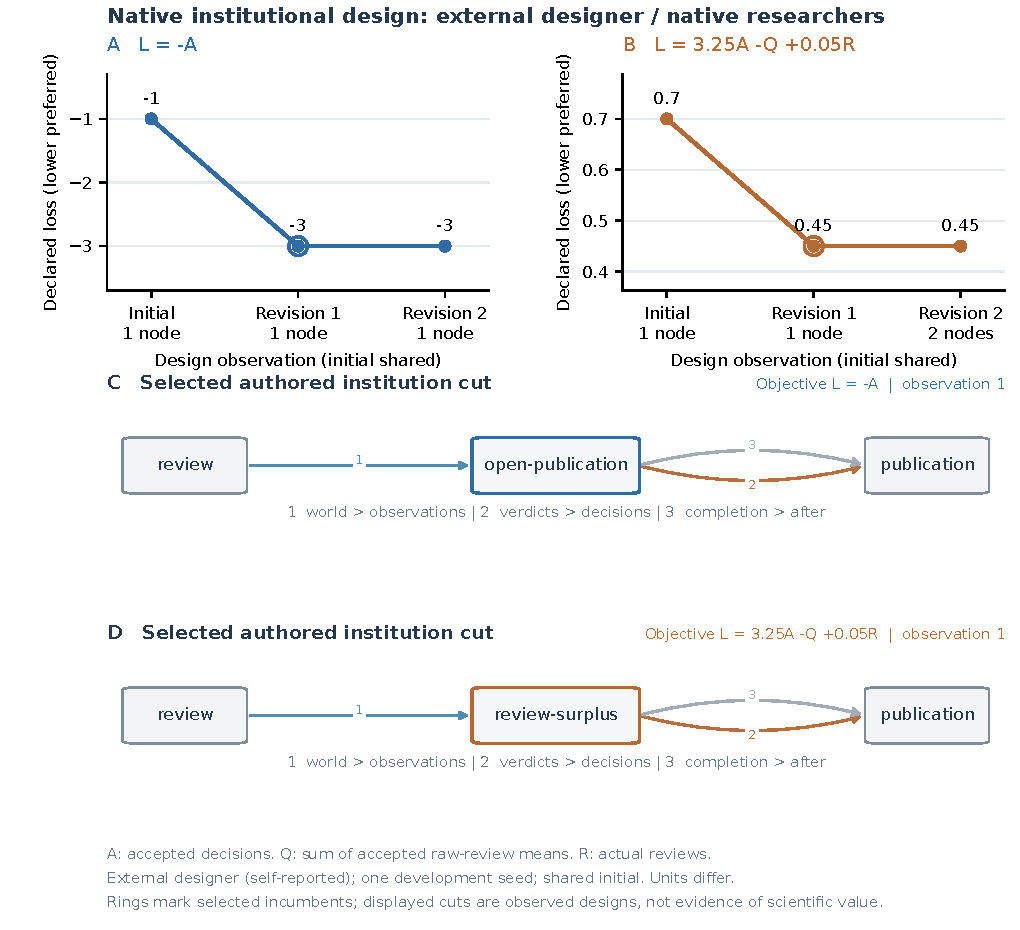
\includegraphics[width=\linewidth]{figures/native-joint-objectives-v5.pdf}
 \caption{Actual objective-conditioned native design with an external Codex
 designer and fixed local Qwen3-8B researchers. A/B: independently audited loss
 paths in different units; node counts refer to the editable cut, not the whole
 scientific system. C/D: exact selected revision-1 cuts. Rings mark the first
 best observation; the later two-node utility revision executes but ties and is
 not the selected graph. One shared physical baseline, four fresh candidates,
 one development seed, five researchers and two years per world. Cross-scoring
 is not held-out evidence; neither all-accept nor all-reject implies good science.}
 \label{fig:native-joint-objectives-v5}
\end{figure}
